\documentclass{beamer}
\usepackage[english]{babel}
\usepackage[utf8]{inputenc}

% AMSLaTeX packages
\usepackage{amsthm}
\usepackage{amsmath}
\usepackage{amsfonts}
\usepackage[algoruled]{algorithm2e}

\usetheme{default}
\useoutertheme{default}
% we want to use images
\usepackage{graphicx}
\usepackage{movie15}
\usepackage{hyperref}

% table relates packages
\usepackage{booktabs}
\usepackage{multirow}
% pick a font
\usepackage{palatino}           
% \usepackage{times}
\usepackage{tikz}
\usetikzlibrary[positioning,arrows,decorations.pathmorphing,backgrounds,fit,calc]
% \AtBeginSection[]  % "Beamer, do the following at the start of every section"
% {
%   \begin{frame}<beamer> 
%     \frametitle{Outline} % make a frame titled "Outline"
%     \tableofcontents[currentsection]  % show TOC and highlight current section
%   \end{frame}                    
% }

% \AtBeginSubsection[]
% {
%   \begin{frame}
%     \frametitle{Outline}
%     \tableofcontents[currentsection,currentsubsection]
%   \end{frame}
% }

\AtBeginSection[]
{
   \begin{frame}
       \frametitle{Outline}
       \tableofcontents[currentsection]
   \end{frame}
}

\newcommand{\ebox}[1][1em]{\framebox[#1]{\phantom{M}}}

\setlength\arraycolsep{1.4pt}% some length

%gets rid of navigation symbols
\setbeamertemplate{navigation symbols}{}

%gets rid of bottom navigation bars
\setbeamertemplate{footline}[page number]{}
\setbeamertemplate{headline}{}


\usebackgroundtemplate{
\includegraphics[width=\paperwidth]{NormalANLBlue}}
\title[LANS Seminar]
{Structure-Exploiting Zeroth-Order Optimization}
\author[Speaker]{\textcolor{red}{By}: Anthony Nguyen \\ \textcolor{red}{Mentors}: Raghu Bollapragada, Matt Menickelly and Stefan M. Wild}
\subtitle{}
\institute[ANL/MCS]{Argonne National Laboratory}
\date{\today}
\begin{document}

\setbeamertemplate{footline}{}
{
\usebackgroundtemplate{
\includegraphics[width=\paperwidth]{TitleANLBlue}}
\frame{\titlepage}
}

\setbeamertemplate{footline}[page number]{}

% FRAME: overview
%\begin{frame}
%  \frametitle{Outlines}
%  \tableofcontents
%\end{frame}
% ========================================
% main slides come here
% ========================================
%\section{Introduction to Problem}
\begin{frame}
  \frametitle{Background}
  \textcolor{red}{Optimization problem}: $\min_{x \in \mathbb{R}^n}\{f(x) = h \circ F(x)\}$ \vspace{0.25in}
  
   \quad \quad where $h(x) = \|x\|^2, F(x) = (F_1(x),\dots,F_p(x))$ \vspace{0.5in}
  
  \textcolor{blue}{Goal}: Minimize $f$ using zeroth order information (using $F(x)$ evaluations and $\nabla F(x)$ unknown). \newline \vspace{0.5in}
  
  
  \textcolor{red}{Question}: Can we exploit $h$ using an efficient algorithm to solve \\ \quad \quad  the optimization problem? 
\end{frame}

%\section{Basic Assumptions}
\begin{frame}
  \frametitle{Assumptions and Gaussian Smoothing}
   %\textcolor{blue}{Unstructured case}: $f: \mathbb{R}^n \to \mathbb{R}$. \\ 
  \textcolor{red}{Structured case}: $f = h \circ F, F: \mathbb{R}^n \to \mathbb{R}^p, f: \mathbb{R}^n \to \mathbb{R}$ \\   \vspace{0.5in}
 
  
	%\textcolor{blue}{Assumptions (unstructured)}: Convexity, smoothness, lipschitz  \\
	\textcolor{red}{Assumptions}: $F$ smooth, $\nabla F_i$ are lipschitz, $f$ is convex, and $\nabla f$ lipschitz. \newline \vspace{0.25in}
	
	\textcolor{red}{Gaussian Smoothing}: 
	 
  \begin{align*}
  f_{\mu}(x) & = \mathbb{E}_{u \sim \mathcal{N}(0,I_n)}[f(x+\mu u)] \\ \nabla f_{\mu}(x) & = \mathbb{E}_{u \sim \mathcal{N}(0,I_n)}\left[\frac{f(x+\mu u)-f(x)}{\mu}u\right]
  \end{align*}
  
 
  %where $\mathbb{E}_u[\psi(u)] = \frac{1}{(2\pi)^{n/2}}\int_{\mathbb{R}^n}\psi(u)e^{-\frac{1}{2}\|u\|^2}du$.
\end{frame}
%\section{Function Estimates}
%\begin{frame}
%  \frametitle{Function Approximation}
%   \textcolor{red}{Gaussian Smoothing}:  $u \sim \mathcal{N}(0,I_n)$, $f: \mathbb{R}^n \to \mathbb{R}$. \newline \vspace{0.25in}
   
%     \textcolor{blue}{Approximations:} $f_{\mu}, \nabla f_{\mu}$ to $f, \nabla f$ by 
%  \begin{align*}
%  f_{\mu}(x) & = \mathbb{E}_u[f(x+\mu u)] \\ \nabla f_{\mu}(x) & = \mathbb{E}_u\left[\frac{f(x+\mu u)-f(x)}{\mu}u\right]
%  \end{align*}
%  where $\mathbb{E}_u[\psi(u)] = \frac{1}{(2\pi)^{n/2}}\int_{\mathbb{R}^n}\psi(u)e^{-\frac{1}{2}\|u\|^2}du$.
%\end{frame}


\begin{frame}
	\frametitle{Estimators}
	
	\textcolor{red}{Draw} $u \sim \mathcal{N}(0,I_n)$. \newline \vspace{0.1in}
	
	\textcolor{blue}{Estimators} $g_{\mu}(x)$ for $\nabla f_{\mu}(x)$: \newline 
	\begin{enumerate}
		\item  $\frac{f(x+\mu u)-f(x)}{\mu}u$
		\item $2F(x+\mu u)^\top\left\{\frac{F(x+\mu u)-F(x)}{\mu}\right\}u$
		\item $2F(x)^\top\left\{\frac{F(x+\mu u)-F(x)}{\mu}\right\}u$
	\end{enumerate}	
	\textcolor{red}{Scheme:} $x_{k+1} = x_k - h g_{\mu}(x_k)$ \\ \vspace{0.25in} 
	\textcolor{blue}{Remark:} Estimator $1$ is unbiased, while estimators $2$ and $3$ are biased for $\nabla f_{\mu}$.

	
	
\end{frame}




%\section{Algorithm}
\begin{frame}
	\frametitle{Structured Algorithm}
\textcolor{red}{Define}: $\mathcal{U}_k = (u_0, \dots, u_k)$, $\phi_0 = f(x_0), \phi_k = \mathbb{E}_{\mathcal{U}_{k-1}}f(x_k)$ \\ \vspace{0.25in}
\textcolor{blue}{Theorem}: Suppose $f$ is convex. If $g_{\mu}$ is an \textbf{unbiased estimator} for $\nabla f_{\mu}$, $h = \frac{1}{4\left(\frac{\mu^2}{2}L_{\nabla F}^2(n+6)^3 + (n+4)L_{\nabla f}\right)} $, and $f^* = 0$, then 
\begin{align*}
\frac{1}{N+1}\sum_{k=0}^N(\phi_k - f^*) & \leq \frac{4(n+4)L_{\nabla f}\|x_0 - x^*\|^2}{N+1} + \mu^2nL_{\nabla f}
\end{align*}

\begin{figure}[ht]
	\centering
	\begin{minipage}[b]{0.45\linewidth}
		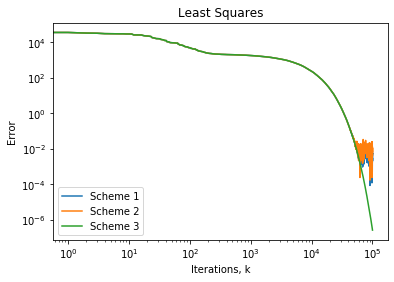
\includegraphics[scale=0.30]{leastSquaresSassy.png}
	\end{minipage}
	\quad
	\begin{minipage}[b]{0.45\linewidth}
		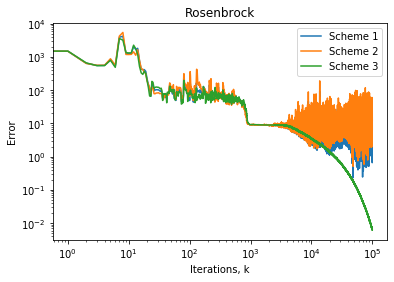
\includegraphics[scale=0.30]{rosenbrockSassy.png}
	\end{minipage}
	\end{figure}

\textcolor{red}{Future Work:} Why biased estimators perform better 
\end{frame}


\end{document}
